% !TeX program = xelatex
% !TeX encoding = UTF-8
\documentclass[withoutpreface,bwprint]{cumcmthesis}
\newcommand{\papertitlemain}{微网与外部电网电力调控策略}
\newcommand{\papertitlesub}{基于因果预测与两日滚动优化的购电及储能调度}
\title{\papertitlemain：\papertitlesub}
\tihao{C}
\baominghao{}
\schoolname{}
\membera{}
\memberb{}
\memberc{}
\supervisor{}
\yearinput{2026}\monthinput{09}\dayinput{13}
\newcommand{\questionconclusion}[1]{\par\medskip\noindent\textbf{本问结论：}#1\par\medskip}
\usepackage{cumcm_official_final}
\usepackage{longtable}
\graphicspath{{sections/}}
\hypersetup{pdftitle={微网与外部电网电力调控策略},pdfsubject={因果预测与两日滚动优化},pdfcreator={XeLaTeX}}
\Urlmuskip=0mu plus 1mu
\newcommand{\R}{\mathbb{R}}
\newcommand{\pos}[1]{\left[#1\right]_+}
\DeclareMathOperator{\clip}{clip}
\begin{document}
\maketitle
\begin{abstract}
针对微网在负荷、光伏与电价变化下的购电调控问题，建立历史预测、两日计划、日内调整与逐槽执行相结合的优化模型。各层明确区分已知预报和未来实际值，以跨日连续储能协调当前供需与次日需求。

问题一建立包含能量平衡、充放电效率、容量及功率界限和日循环条件的线性规划。典型日最优购电量为59482.7 kWh，费用35126.95元，较无储能基线节省26.9\%。

问题二以历史实现费用标定三源凸组合预测，采用半衰期5天的指数加权更新。开发期选定负荷抬升系数1.02与光伏折减25 kW，每天优化两日、执行首日，实际日末电量自由并跨日传递。2月至12月共334天总费用为1395.7万元，其中紧急购电费79.6万元。固定计划的联合残差重采样显示，总成本均值1464万元，P95为1542万元。

问题三将官方光伏预报与历史预测按0.7和0.3组合，在6、12、18时调整未执行计划，并在前两次调整引入40个联合残差情景。主方案费用1349.2万元，较官方预报无调整基线下降7.87\%。消融中无对冲方案费用1347.1万元，表明当前数据支持日内调整和组合预测的价值，但尚不支持对冲的实现费用优势。

问题四将价格替换为给定波动电价，两层策略费用分别为1459.8和1412.6万元。仅用历史价格预测的扩展费用为1465.9和1420.5万元，对应额外成本0.42\%和0.56\%。

情景数、种子与历史池扰动下结果总体稳定，约束残差达到浮点误差量级，跨日SOC连续且场景池无前视。模型同时说明初始状态、单年样本与分层规划近似的适用边界，为微网购电和储能运行提供可复现的决策依据。
\keywords{微网调度；两日滚动；因果预测；储能优化；日内调整；联合残差情景}
\end{abstract}

\section{问题重述}
\subsection{研究背景}
小区微网通过光伏发电、储能电池和外部购电共同满足负荷。电池能够将低价时段的电能转移到高价时段，也能够吸收光伏富余电量；但预测偏差会使计划与实际需求不匹配，导致额外购电或弃电。因而，调度问题不仅是寻找一条低成本的购电曲线，还要使这条曲线在信息逐步到达的条件下可执行。
\subsection{四个问题的递进关系}
问题一依据典型日电价、负荷与光伏预测，建立当天购电及储能调度模型，要求日初、日末电量相同，并给出指定时段结果。问题二考虑逐日变化的负荷和光伏，要求每天零点作出购电计划，实际短缺按当期五倍电价紧急购电，常规购电按计划结算。
问题三允许利用零点及6、12、18时发布的光伏预报制定和调整计划，调整还会产生相对原计划的偏差费用，需要同时评价新增信息和调整时机的作用。
问题四进一步考虑波动电价，分别重算无日内调整与有日内调整两种策略。
本文在共同的储能约束下逐步改变信息集与结算目标，使四问结果具有清晰的比较基础。

\section{数据理解与总体分析}
\subsection{数据处理与评价区间}
附件1给出144个10分钟时段的典型日电价、负荷和光伏；附件2给出2025年实际负荷与光伏；附件3给出每天四次发布的24小时光伏预报；附件4给出波动电价。本文以电量为优化变量，功率乘$\Delta t=1/6$小时后统一为kWh，电价保持元/kWh。
附件与结果模板的时间文字存在一个10分钟刻度差异，因此输出沿用模板标签，以行列序号一一对应原始槽数据，避免因字符串匹配造成错位。本文指定时段表也沿用结果模板标签。

附件3中提前$k$小时的值对应发布时刻加$k$小时，故每次更新都按发布时刻重建时间轴，再插值至10分钟粒度。6、12、18时预报只用于该次发布之后尚未执行的时段，不能直接套用零点预报的映射。
负荷与光伏历史预测均仅使用决策日前的实际值；典型日曲线视为题目给定的外生参考资料，不从完整年度实际值重新计算。

根据结果模板，问题二至四统一评价2025年2月1日至12月31日，共334天。1月数据用于形成滞后特征与预热权重。当前实验在2月1日以6000 kWh初始化储能；这是评价区间的统一初始条件，并非对1月运行后的储电量进行推导。题面给出1月1日初值，因此本文结果应理解为指定报送区间的条件回测，初始状态的局限在模型评价中讨论。

\subsection{误差结构与决策目标}
数据分析表明，光伏光照样本的预测误差随提前时间增加，近似关系为
$\mathrm{MAE}(k)\approx14.8+29.0k$ kW，拟合$R^2=0.982$。
下午13至18时的光伏MAE随发布时刻由零点推进至6时、12时，从413 kW降至248 kW、76 kW。
日内误差的前四阶相关系数为0.79、0.60、0.40、0.21，说明逐点独立扰动会破坏误差的时间结构。
因此，日内更新预报具有调度价值；整日联合残差场景作为候选扩展，通过消融决定是否进入正式方案。

紧急购电与计划购电的价格不对称，最小预测均方误差并不直接等于最小购电成本。
本文用历史实现费用标定预测组合，在名义预测上加入小幅保守修正，再利用当前实际状态逐槽执行。
候选场景法保留负荷和光伏残差的同日联合结构，避免只考虑光伏误差而遗漏净负荷风险；若留出实验不支持，则按简约原则删除。

\subsection{两日规划与滚动执行}
每天零点优化当日与次日共288个槽，只承诺首日计划；次日计划是储能机会成本的近似参考，到次日零点会重新计算。该思路借鉴滚动时域优化\cite{mayne2000}，但本文采用的有限窗口与实时执行规则并不具有自动成立的无限时域最优性保证。
问题三在日内预报发布时重算剩余时段，执行层每10分钟只读取当前实际值，日末储电量自然传递至次日。
表\ref{tab:info}概括不同问题的信息范围。
\begin{table}[htbp]\centering
\caption{各问题的信息集与调度结构}\label{tab:info}
\small
\begin{tabularx}{\textwidth}{c X X X}
\toprule
问题 & 零点负荷与光伏输入 & 电价输入 & 调整与储能结构\\
\midrule
一 & 典型日给定数据 & 典型日给定 & 单日规划、日循环\\
二 & 因果历史预测 & 典型日电价 & 无日内调整、两日滚动\\
三 & 历史负荷与组合光伏预报 & 典型日电价 & 三次更新、跨日连续\\
四 & 分别沿用问题二、三预测 & 给定波动电价G & 分别重算两层策略\\
扩展H & 与问题四对应层一致 & 历史价格预测 & 评价电价信息价值\\
\bottomrule
\end{tabularx}
\end{table}

\subsection{统一求解框架}
四问共用同一套“预测—计划—调整—执行—结算”框架，仅在题面允许的信息集与结算目标上存在差异。
图\ref{fig:corealg}给出该统一核心算法：每天零点先用决策日前的实际值构造负荷与光伏的自适应组合预测
（问题三、四在光伏上另与官方预报组合），权重按历史实现费用以指数加权方式逐日标定；
对预测施加负荷抬升与光伏折减的保守裕度后，求解当日与次日共288个槽的购电与储能线性规划，
规划窗口末端自由，只承诺首日计划。问题三与问题四在6、12、18时以最新发布的预报和当时的
实际储电量重算剩余时段，调整量按调低部分付50\%、调高部分付150\%的规则产生偏差费用；
执行层逐槽读取当前已实现的负荷与光伏，缺口按当期电价5倍紧急购电，富余只能弃光，
日末储电量自然传递至次日并触发滚动重解。问题一为确定性特例，采用单日循环模型；
问题四仅将价格输入替换为附件4的波动电价。图中每一环节的“口径”行汇总了对应问题的信息集差异。
\begin{figure}[htbp]\centering
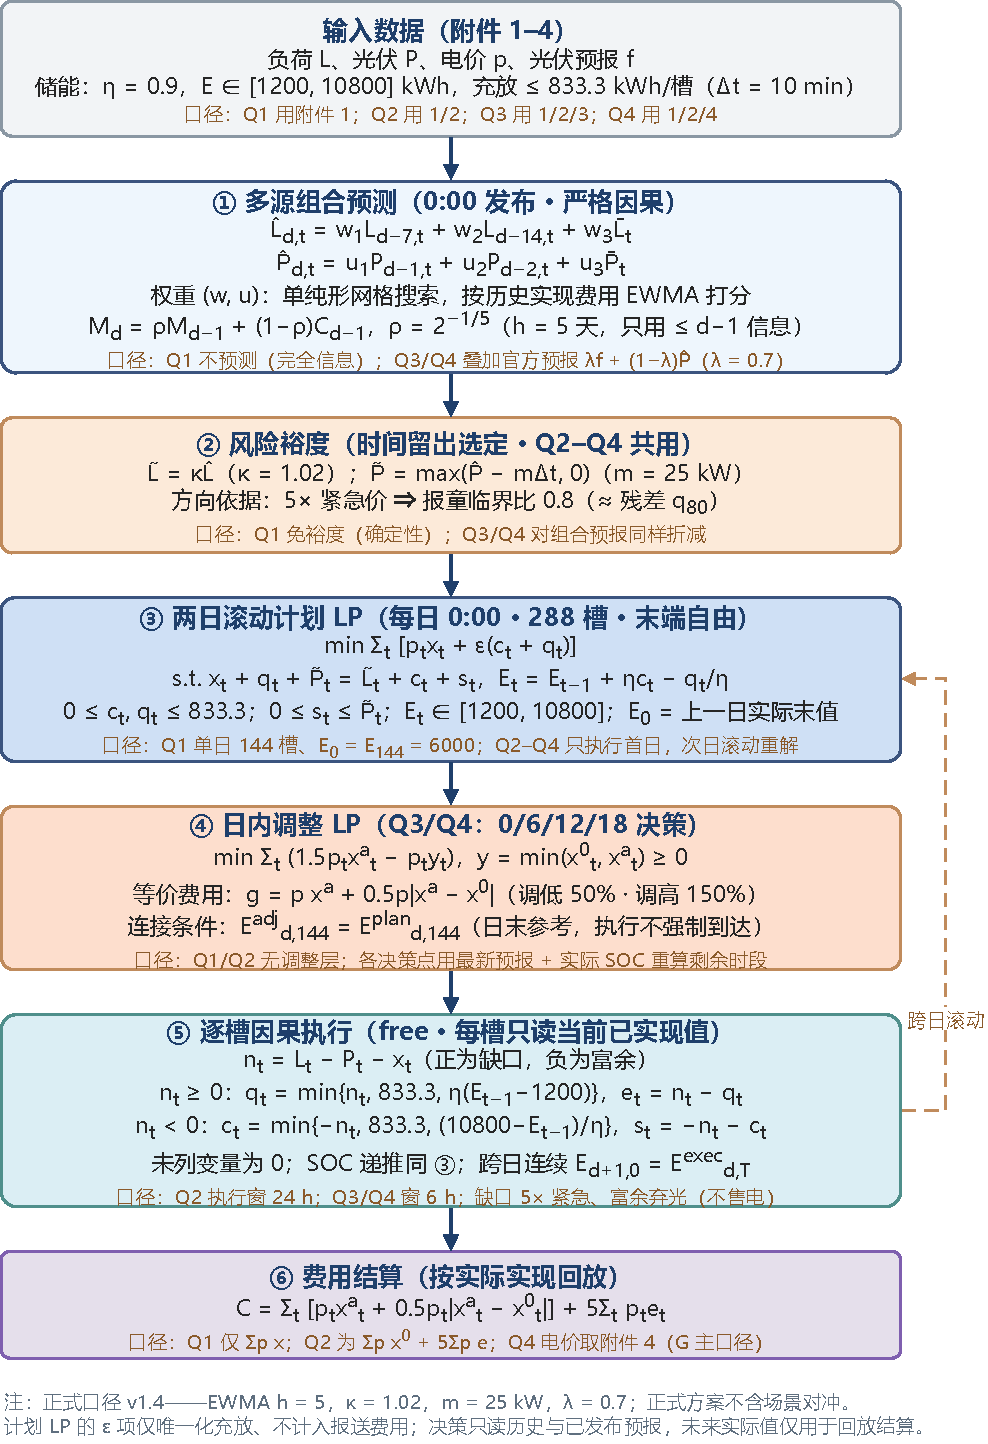
\includegraphics[width=.9\textwidth]{../../figures/核心算法流程图.pdf}
\caption{Q1--Q4共用的统一核心算法流程（含各问信息集差异与结算口径）}\label{fig:corealg}
\end{figure}

\section{模型假设}
\begin{enumerate}
\item 每10分钟内功率按常数近似，负荷不可主动削减。该假设使连续能量平衡转化为有限维线性约束。
\item 储能充电和放电各按90\%效率计损，往返效率为81\%；不另计自放电与寿命衰减。该解释适用于题目给定的固定效率条件。
\item 微网不售电；无法被负荷或储能吸收的供给可弃置。预测规划中的弃光和执行中计划购电富余的弃电应区别理解，后者不获得退款。
\item 常规购电按已承诺电量结算，短缺额外以五倍当期价格采购。问题三各槽按最终有效调整量相对零点原计划结算一次，避免对同一槽重复计收偏差费用。
\item 问题一保留题面要求的日循环；问题二至四不人为固定每日实际末端电量，两日规划最远端仅受容量边界约束。日内调整规划的末端参考由当日两日计划内生给出，执行允许偏离该参考。
\item 波动电价主分析G将附件4给定价格作为规划窗口内已知输入；H作为仅有历史价格的扩展。G不是对未来实际负荷或光伏已知的假设。
\end{enumerate}

\section{符号说明}
\begin{table}[htbp]\centering
\caption{主要符号、含义与单位}\label{tab:symbol}
\small
\begin{tabularx}{\textwidth}{p{.20\textwidth}Xp{.15\textwidth}}
\toprule
符号 & 含义 & 单位\\\midrule
$d,t;\ T,H$ & 日期、日内槽；日槽数144、规划槽数288 & ---\\
$L_{d,t},P_{d,t}$ & 实际负荷、光伏电量 & kWh\\
$\widehat L,\widehat P$ & 决策时刻可得的预测电量 & kWh\\
$p_{d,t}$ & 交易电价 & 元/kWh\\
$x^0_{d,t},x^a_{d,t}$ & 零点计划、各槽最终有效调整购电量 & kWh\\
$c_{d,t},q_{d,t}$ & 充入、放出的电网侧电量 & kWh\\
$E_{d,t}$ & 时段末储能电量 & kWh\\
$e_{d,t},s_{d,t}$ & 紧急购电量、富余弃电量 & kWh\\
$\eta,\bar c$ & 单向效率0.9、单槽充放上限$5000/6$ & ---、kWh\\
$w_d,u_d$ & 历史负荷、光伏的三源凸组合权重 & ---\\
$h,\kappa,m$ & EWMA半衰期、负荷抬升、光伏折减 & 天、---、kW\\
$\lambda,S$ & 官方光伏预报占比、情景数 & ---\\
$\mathcal I_{d,t}$ & 决策时刻已获得的信息集合 & ---\\
\bottomrule
\end{tabularx}
\end{table}
带上标$s$的变量表示第$s$个情景，$[z]_+=\max(z,0)$。下文未列出的局部辅助变量在首次出现时定义。

\section{问题一：典型日确定性储能调度}
\subsection{线性规划模型}
对给定的典型日，决策变量为购电$x_t$、充电$c_t$、放电$q_t$、电量$E_t$及弃光$s_t$。
在不需要紧急购电的确定性条件下，目标为
\begin{equation}\min C_1=\sum_{t=1}^{T}p_tx_t.\label{eq:q1obj}\end{equation}
每个槽满足供需平衡与储能递推：
\begin{align}
P_t+x_t+q_t&=L_t+c_t+s_t,\label{eq:balance}\\
E_t&=E_{t-1}+\eta c_t-q_t/\eta.\label{eq:soc}
\end{align}
充电量从电网侧计量，故进入电池的电量为$\eta c_t$；向负荷放出$q_t$需消耗$q_t/\eta$。
容量、功率、非负性与循环条件为
\begin{align}
1200\leq E_t\leq10800,\quad &0\leq c_t,q_t\leq5000/6,\label{eq:bounds}\\
x_t\geq0,\quad 0\leq s_t\leq P_t,\quad &E_0=E_T=6000.\label{eq:cycle}
\end{align}
所有约束与目标均为线性，共720个变量、289条等式约束，采用稀疏矩阵和HiGHS求解。
线性规划算法可高效求解该规模问题\cite{huangfu2018}。模型未引入充放互斥二元变量，因此解后必须检查同槽同时充放；所得正式解通过该项检查。
\subsection{最优策略与题目指定结果}
最优全天购电量为59482.7 kWh，购电费为35126.95元，较无储能基线节省26.9\%。
电池利用低价时段充电，在高价及光伏不足时段释放电能，全天弃光为0。
题面指定的购电及储能结果列于表\ref{tab:q1buy}、表\ref{tab:q1soc}。
\begin{table}[htbp]\centering
\caption{问题一指定时段购电量（kWh）}\label{tab:q1buy}
\small
\begin{tabular}{cr}
\toprule
时间段 & 购电量 \\
\midrule
10:00-10:10 & 0.00 \\
12:00-12:10 & 486.40 \\
14:00-14:10 & 0.00 \\
16:00-16:10 & 394.93 \\
18:00-18:10 & 636.98 \\
20:00-20:10 & 0.00 \\
\midrule 全天购电量 & 59482.7 \\
全天购电费/元 & 35126.95 \\
\bottomrule
\end{tabular}
\end{table}
\begin{table}[htbp]\centering
\caption{问题一指定区间储能充放电量（kWh）}\label{tab:q1soc}
\small
\begin{tabular}{crr}
\toprule
时间段 & 充电量 & 放电量 \\
\midrule
0:00-4:00 & 4500.00 & 0.00 \\
4:00-8:00 & 833.33 & 6365.84 \\
8:00-12:00 & 4787.96 & 1703.00 \\
12:00-16:00 & 5286.04 & 91.10 \\
16:00-20:00 & 0.00 & 5780.13 \\
20:00-24:00 & 5333.33 & 2859.87 \\
\midrule 0:00储电量 & \multicolumn{2}{c}{6000.00} \\
24:00储电量 & \multicolumn{2}{c}{6000.00} \\
\bottomrule
\end{tabular}
\end{table}

\begin{figure}[htbp]\centering
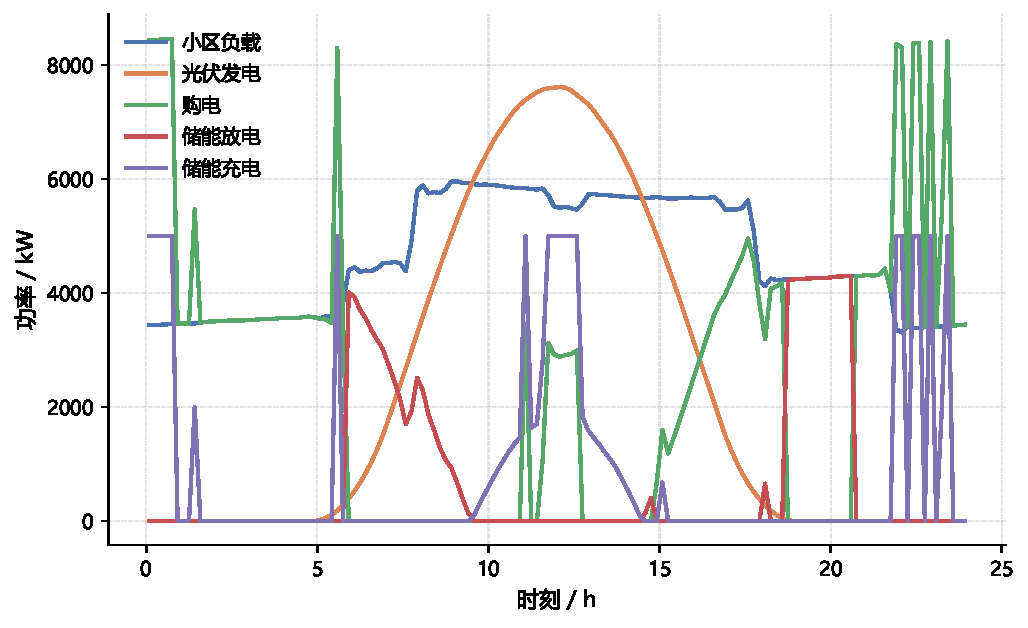
\includegraphics[width=.92\textwidth]{../../figures/Q1_调度时序.pdf}
\caption{典型日购电、光伏与储能联合调度}\label{fig:q1}
\end{figure}
图\ref{fig:q1}中的充放电时序同时受峰谷价格和光伏出力影响。由于循环条件约束日末电量，全天节省不是通过消耗初始储能获得的暂时收益。
四小时汇总区间内可能同时出现正的累计充电与放电量，这表示不同10分钟槽采用不同动作，不意味着同槽同时充放。
\questionconclusion{确定性典型日最优购电费为35126.95元，储能节省比例26.9\%；该模型提供后续各问共用的物理约束。}

\section{问题二：历史预测与两日滚动购电}
\subsection{面向费用的历史组合预测}
在零点尚不知道当天实际负荷与光伏，因此根据周周期与短期持续性构造
\begin{align}
\widehat L_{d,t}&=w_{d,1}L_{d-7,t}+w_{d,2}L_{d-14,t}+w_{d,3}\bar L_t,\label{eq:load}\\
\widehat P_{d,t}&=u_{d,1}P_{d-1,t}+u_{d,2}P_{d-2,t}+u_{d,3}\bar P_t,\label{eq:pv}
\end{align}
其中$\bar L_t,\bar P_t$为题目给定典型日电量，权重非负且各自和为1。
两组三源权重在步长0.2的单纯形网格搜索，共$21\times21=441$个组合。
令$C_j(w,u)$为历史日$j$使用该权重作计划并以实际值因果执行后的总费用，递推评分为
\begin{equation}
\begin{aligned}
M_d(w,u)&=\rho M_{d-1}(w,u)+(1-\rho)C_{d-1}(w,u),\\
\rho&=2^{-1/h},\qquad (w_d,u_d)=\arg\min_{w,u}M_d(w,u).
\end{aligned}
\label{eq:ewma}
\end{equation}
历史首个可用评分初始化$M$，随后每日只吸收前一日实现费用。半衰期取$h=5$天。
历史成本表采用单日规划、自由末端执行的代理费用，正式运行采用两日滚动，二者不能视为完全相同的优化目标；这种代理降低了逐日权重标定的计算量。

为控制高价短缺，对预测施加
\begin{equation}
\widetilde L_{d,t}=\kappa\widehat L_{d,t},\qquad
\widetilde P_{d,t}=[\widehat P_{d,t}-m\Delta t]_+,
\quad \kappa=1.02,\ m=25\ {\rm kW}.
\label{eq:margin}
\end{equation}
若忽略储能与跨期耦合，仅考虑计划量$z$和随机净需求$N$，最小化
$pz+5p\,\mathbb E[(N-z)_+]$给出$F_N(z)=0.8$。
这解释了保守修正的方向，但不能据此直接确定含储能模型的最优裕度；具体参数仍由历史开发期费用选择。
\subsection{两日计划及次日预测}
每日以实际日初电量$E_{d,0}$初始化288槽规划，目标为
\begin{equation}
\min\sum_{\tau=1}^{288}\widehat p_\tau x_\tau+
\varepsilon\sum_{\tau=1}^{288}(c_\tau+q_\tau),
\label{eq:rolling}
\end{equation}
并对预测负荷、光伏施加式\eqref{eq:balance}--\eqref{eq:bounds}。
微小吞吐量正则项用于减少无意义充放循环，报送购电费不含此数值求解罚项。
当日末$E_{144}$和窗口最远端$E_{288}$均不设置等式终值，仅满足容量界限。
次日负荷利用$d+1-7,d+1-14$的已发生曲线，当日冻结的光伏权重应用于截至$d-1$的最近两条实际曲线；禁止使用当天尚未发生的光伏来构造次日预测。
\subsection{逐槽因果执行}
固定当前有效承诺量$x_t$，观察当前实际负荷和光伏，记
$n_t=L_t-P_t-x_t$。当$n_t\geq0$时，
\begin{equation}
q_t=\min\{n_t,\bar c,\eta(E_{t-1}-1200)\},\quad
e_t=n_t-q_t,\quad c_t=s_t=0.
\label{eq:discharge}
\end{equation}
当$n_t<0$时，
\begin{equation}
c_t=\min\{-n_t,\bar c,(10800-E_{t-1})/\eta\},\quad
s_t=-n_t-c_t,\quad q_t=e_t=0.
\label{eq:charge}
\end{equation}
然后按式\eqref{eq:soc}更新储电量。这一规则只依赖当前槽及此前信息，不为追赶日末目标而额外紧急购电充能。
次日初值为本日实际末值：
\begin{equation}E_{d+1,0}=E_{d,T}^{\rm exec}.\label{eq:crossday}\end{equation}
计划富余不会退费，故实现费用为
\begin{equation}C_2=\sum_d\sum_t p_t x^0_{d,t}+5\sum_d\sum_t p_t e_{d,t}.\label{eq:q2cost}\end{equation}
\subsection{时间留出选择与总费用}
2月至6月为开发期，7月至12月为验证期；后者只报告性能，不用于重新选择全局参数。
表\ref{tab:holdout}显示相邻候选表现接近。所选$m=25$在开发期最优，在验证期排名第5；$m=50$的全年描述值略低，也不能据此倒过来改选。
因此334天汇总包括开发期，不能称为全区间独立样本外测试。
\begin{table}[htbp]\centering
\caption{问题二部分候选的时间留出结果（万元，均为$h=5$）}\label{tab:holdout}
\begin{tabular}{ccrrrr}
\toprule
$\kappa$ & $m$/kW & 开发期 & 验证期 & 全区间 & 验证排名\\\midrule
1.02 & 25（选定） & 574.0 & 821.6 & 1395.7 & 5\\
1.02 & 50 & 574.2 & 820.6 & 1394.8 & 4\\
1.015 & 75 & 574.3 & 821.7 & 1396.1 & 6\\
1.02 & 75 & 575.0 & 820.3 & 1395.3 & 2\\
\bottomrule
\end{tabular}
\end{table}
正式结果总费用1395.7万元，其中计划购电费1316.0万元、紧急购电费79.6万元；分项独立舍入可能与总额相差0.1万元。
图\ref{fig:q2soc}给出储能轨迹，日末值随供需变化而变化，验证了跨日状态连续与非固定末端条件。
\begin{figure}[htbp]\centering
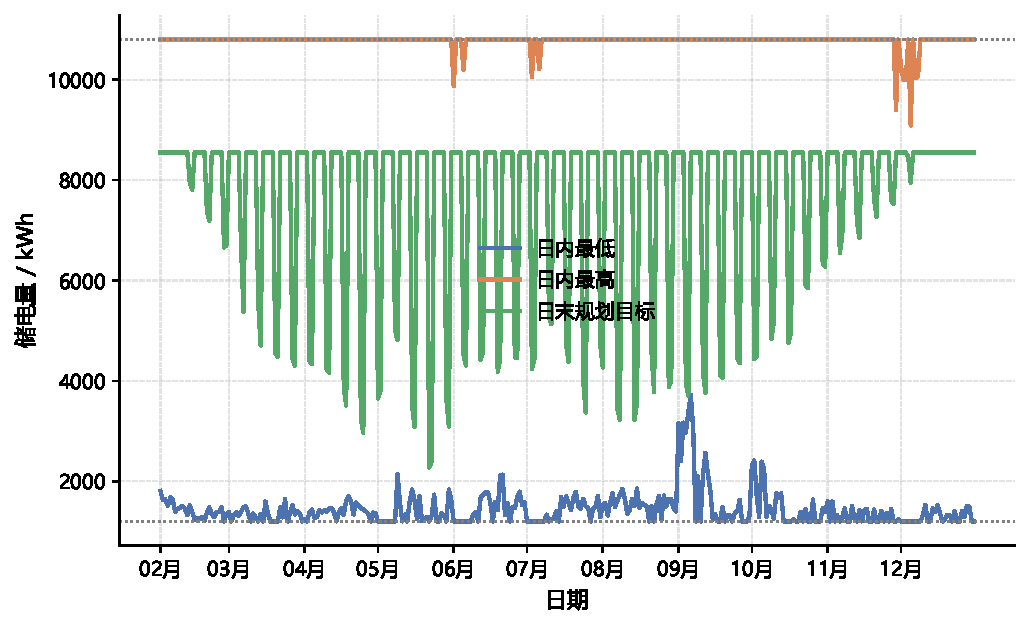
\includegraphics[width=.91\textwidth]{../../figures/Q2_储能轨迹.pdf}
\caption{问题二实际储能电量及日末电量变化}\label{fig:q2soc}
\end{figure}
\subsection{指定日期结果与年度风险}
四个指定日期的计划购电、储能与紧急购电结果见表\ref{tab:q2buy}--\ref{tab:q2emerg}。
计划购电费与包含紧急费的总费用分别列示，以保持题目结算含义。
\begin{table}[htbp]\centering
\caption{问题二指定日期计划购电量与购电费}\label{tab:q2buy}
\small
\begin{tabular}{lrrrr}
\toprule
时段或指标 & 3月20日 & 6月21日 & 9月23日 & 12月21日 \\
\midrule
10:00-10:10 & 0.00 & 0.00 & 0.00 & 0.00 \\
12:00-12:10 & 529.03 & 0.00 & 553.22 & 975.48 \\
14:00-14:10 & 0.00 & 0.00 & 0.00 & 0.00 \\
16:00-16:10 & 428.10 & 169.90 & 464.46 & 796.72 \\
18:00-18:10 & 744.10 & 534.28 & 802.45 & 731.57 \\
20:00-20:10 & 0.00 & 0.00 & 0.00 & 0.00 \\
全天计划电量/kWh & 62281.59 & 42865.34 & 69038.87 & 96267.73 \\
全天计划购电费/元 & 38733.07 & 24447.24 & 42750.14 & 61810.51 \\
紧急购电费/元 & 1592.53 & 0.00 & 1003.07 & 83.06 \\
含紧急费总额/元 & 40325.60 & 24447.24 & 43753.21 & 61893.57 \\
\bottomrule
\end{tabular}
\end{table}
\begin{table}[htbp]\centering
\caption{问题二指定日期储能充放电与首末电量（kWh）}\label{tab:q2soc}
\footnotesize
\setlength{\tabcolsep}{4pt}
\begin{tabular}{lrrrrrrrr}
\toprule
 & \multicolumn{2}{c}{3月20日} & \multicolumn{2}{c}{6月21日} & \multicolumn{2}{c}{9月23日} & \multicolumn{2}{c}{12月21日}\\
区间 & 充电 & 放电 & 充电 & 放电 & 充电 & 放电 & 充电 & 放电 \\
\midrule
0:00-4:00 & 1376.88 & 122.05 & 447.73 & 200.31 & 2042.44 & 43.58 & 2040.21 & 276.70 \\
4:00-8:00 & 992.89 & 4988.27 & 593.50 & 1782.09 & 405.75 & 6608.26 & 1608.84 & 1579.87 \\
8:00-12:00 & 5356.38 & 2777.38 & 7656.06 & 0.00 & 5589.93 & 1896.62 & 5310.48 & 7513.53 \\
12:00-16:00 & 4272.48 & 534.09 & 0.00 & 0.00 & 5123.65 & 597.06 & 7804.74 & 2276.46 \\
16:00-20:00 & 313.91 & 5924.64 & 242.20 & 5524.96 & 213.59 & 5649.98 & 0.00 & 5685.08 \\
20:00-24:00 & 4089.80 & 2792.53 & 8635.18 & 2570.34 & 8474.10 & 2826.51 & 8405.16 & 2848.38 \\
0:00电量 & \multicolumn{2}{c}{9061.33} & \multicolumn{2}{c}{5175.11} & \multicolumn{2}{c}{8709.06} & \multicolumn{2}{c}{8652.78} \\
24:00电量 & \multicolumn{2}{c}{4780.15} & \multicolumn{2}{c}{9794.87} & \multicolumn{2}{c}{8793.57} & \multicolumn{2}{c}{8883.03} \\
\bottomrule
\end{tabular}
\end{table}
\begin{table}[htbp]\centering
\caption{问题二指定日期全部紧急购电事件}\label{tab:q2emerg}
\small
\begin{tabular}{ccr}
\toprule
日期 & 紧急购电时段 & 紧急购电量/kWh \\
\midrule
03月20日 & 20:30-20:40 & 228.2867 \\
06月21日 & 无 & 0.0000 \\
09月23日 & 20:20-20:40 & 103.1061 \\
09月23日 & 20:50-21:10 & 43.2148 \\
09月23日 & 21:20-21:40 & 17.9760 \\
12月21日 & 7:50-8:00 & 14.2992 \\
\bottomrule
\end{tabular}
\end{table}

固定已生成的两日滚动计划，对负荷和光伏联合残差作同月整日块重采样，得到100个模拟评价年度。
这种模拟是条件于固定计划的离线压力评估，不是重新训练并逐年适应的独立样本外试验。
总成本均值1464万元，标准差44.53万元，P95为1542万元，尾部均值CVaR95为1566万元。
CVaR刻画超过分位阈值的平均损失\cite{rockafellar2000}，适合补充均值指标。
\begin{figure}[htbp]\centering
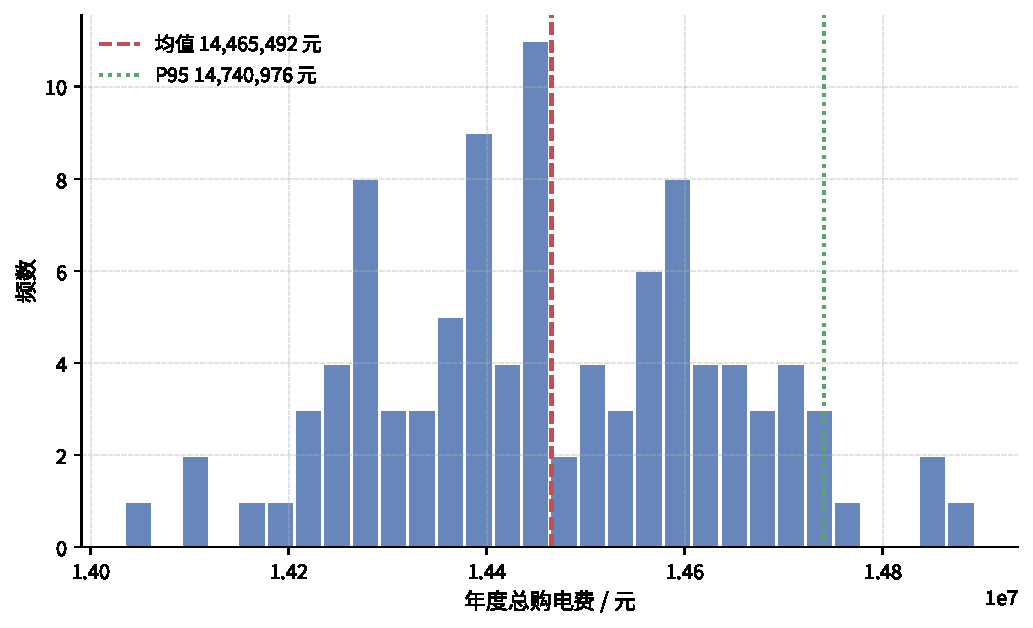
\includegraphics[width=.75\textwidth]{../../figures/Q2_总费用分布.pdf}
\caption{固定计划下联合残差重采样的总费用分布}\label{fig:q2risk}
\end{figure}
图\ref{fig:q2risk}表明实际评价区间的1395.7万元低于重采样均值，不能把这一实现值直接等同于未来期望成本。
\questionconclusion{基于开发期选择的历史预测与两日滚动策略在334天内产生1395.7万元费用；实际末端电量自由，风险评价仍显示明显的高费用尾部。}

\section{问题三：组合预报与日内调整}
\subsection{统一发布相位的组合预报}
零点计划层以及各调整时刻$r\in\{6,12,18\}$均采用
\begin{equation}
\widetilde P^{(r)}_{d,t}=
\left[\lambda\widehat P^{\,\mathrm{off},r}_{d,t}
+(1-\lambda)\widehat P^{\,\mathrm{hist}}_{d,t}-m\Delta t\right]_+,
\quad \lambda=0.7.
\label{eq:mix}
\end{equation}
官方预报使用对应发布时刻的曲线，历史项与问题二一致；负荷继续使用因果历史预测和$\kappa=1.02$修正。第二日尚无对应零点官方预报，使用零点可得的历史外推。
采用相同组合形式的目的，是使日内更新仅反映新信息，而不同时改变预测构造。

\subsection{调整费用的等价表达}
对某个尚未执行的槽，设原计划为$x^0$、最终调整量为$x^a$。
当$x^a\leq x^0$，购电加违约费用为$px^a+0.5p(x^0-x^a)$；
当$x^a>x^0$，费用为$px^0+1.5p(x^a-x^0)$。二者统一为
\begin{equation}
g(x^a;x^0)=px^a+0.5p|x^a-x^0|.
\label{eq:adjustcost}
\end{equation}
因此不能将原计划费用再完整相加，否则会重复计费。
引入$y\leq x^0,\ y\leq x^a,\ y\geq0$，则
$g=1.5px^a-py+0.5px^0$在最优时成立。
最后一项对调整决策是常数，可在求解时省略，但费用统计必须恢复。

\subsection{名义调整与日末参考}
每次新预报发布后，以当前实际SOC初始化剩余时段规划，已执行时段不再修改。
零点两日规划产生当日末的参考电量$E^{\rm ref}_{d,T}=E^{\rm plan}_{d,144}$。
当前日内调整LP保留
\begin{equation}
E^{\rm adj}_{d,T}=E^{\rm ref}_{d,T}
\label{eq:adjterminal}
\end{equation}
作为规划连接条件；该参考由每日预测、价格与日初状态共同决定，并非恒定6000 kWh。
实际执行仍用式\eqref{eq:discharge}--\eqref{eq:charge}，不强制到达此参考。
因而必须区分“规划采用动态日末参考”和“实际日末电量自由”。
这种分层连接保留了次日储能需求的部分信息，但日内层尚未直接重算完整两日窗口，属于模型近似。

\subsection{联合场景候选扩展}
为检验随机规划能否进一步降低短缺风险，先构造一个对冲候选扩展。
在6时和12时，从目标日之前的最近90天中选择残差池；其中同月样本达到14天时优先使用同月样本。
对历史日$j<d$，用其对应发布时刻的名义预测构造联合残差
\begin{equation}
R^L_{j,t}=L_{j,t}-\widetilde L_{j,t},\qquad
R^{P,r}_{j,t}=P_{j,t}-\widetilde P^{(r)}_{j,t}.
\label{eq:residual}
\end{equation}
同一场景的负荷和光伏取自同一天，并保留整段曲线。
每次调整使用$S=40$个等权情景，包含1个名义情景及39个有放回重采样情景；两次调整共抽样78个残差日索引，并不表示每次有78个场景。

不同情景共享调整量$x^a$，各自拥有充放电、弃电、储能与紧急补救变量。
对剩余时段集合$\mathcal T_r$，求解
\begin{equation}
\min\ \sum_{t\in\mathcal T_r}(1.5p_tx^a_t-p_ty_t)
+\frac1S\sum_{s=1}^S\sum_{t\in\mathcal T_r}
\left[5p_te^s_t+\varepsilon(c^s_t+q^s_t)\right],
\label{eq:scenarioobj}
\end{equation}
约束为各情景下的能量平衡、SOC动态、容量与功率界限，以及式\eqref{eq:adjterminal}和$y$的线性化约束。
目标中的$1/S$不可省略，否则情景数增加等价于人为提高紧急费权重。
18时采用名义剩余时段调整；这是一项计算与信息价值折中，并不意味着18时以后完全没有负荷不确定性。

场景内的补救轨迹仅服务于计划评价，其拥有的整段情景信息不等于实际执行可提前获知未来。
候选扩展的实现费用也一律用逐槽因果执行回放计算：
\begin{equation}
C_3=\sum_{d,t}\left[p_tx^a_{d,t}+0.5p_t|x^a_{d,t}-x^0_{d,t}|+5p_te_{d,t}\right].
\label{eq:q3cost}
\end{equation}
正式方案则不求解式\eqref{eq:scenarioobj}，在每个发布时刻只按最新组合名义预测调整剩余计划。
这样既保留相同的信息结构和动态日末参考，又消除了场景抽样及完整情景补救带来的额外保守性。
\subsection{整体表现与指定日期结果}
正式主方案334天总费用1347.1万元，其中计划费1290.5万元、调整净额25.2万元、紧急费31.4万元。
此处调整净额定义为$\sum[g(x^a;x^0)-px^0]$，不是绝对偏差费本身。
与官方预报无调整基线1464.5万元相比，费用降低8.01\%；与官方预报三点调整1357.5万元相比降低0.76\%。
图\ref{fig:q3compare}说明主要收益来自允许更新和调整，组合预测进一步小幅改善费用。
\begin{figure}[htbp]\centering
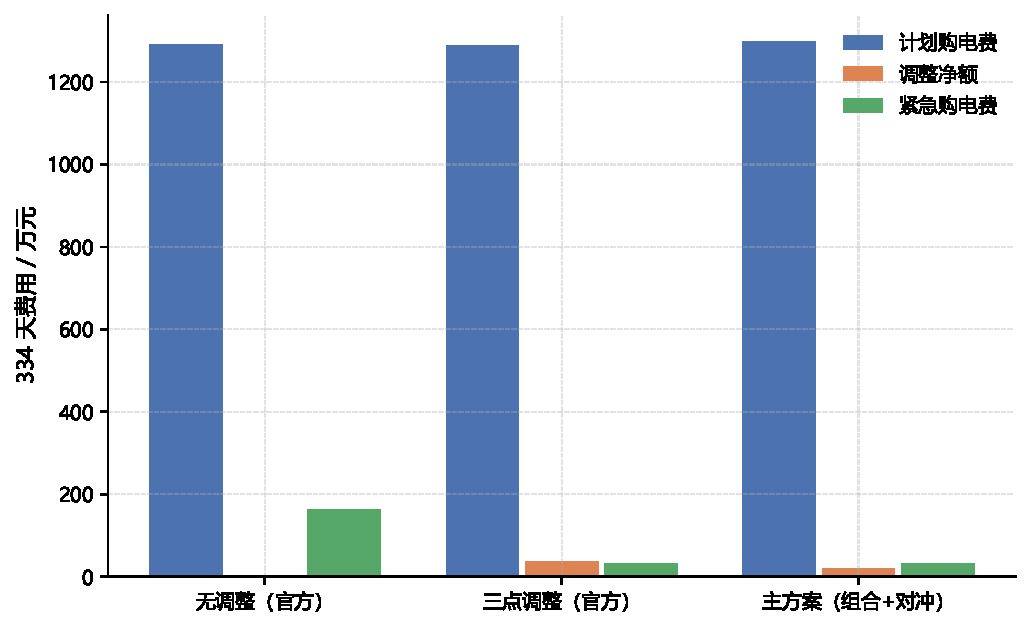
\includegraphics[width=.85\textwidth]{../../figures/Q3_策略费用对比.pdf}
\caption{问题三不同信息与调整策略的费用分解}\label{fig:q3compare}
\end{figure}
\begin{table}[htbp]\centering
\caption{问题三指定日期计划购电量与购电费}\label{tab:q3buy}
\small
\begin{tabular}{lrrrr}
\toprule
时段或指标 & 3月20日 & 6月21日 & 9月23日 & 12月21日 \\
\midrule
10:00-10:10 & 0.00 & 0.00 & 0.00 & 0.00 \\
12:00-12:10 & 567.21 & 0.00 & 419.53 & 966.15 \\
14:00-14:10 & 0.00 & 0.00 & 0.00 & 0.00 \\
16:00-16:10 & 618.29 & 187.98 & 586.23 & 811.78 \\
18:00-18:10 & 706.57 & 0.00 & 787.06 & 735.24 \\
20:00-20:10 & 0.00 & 0.00 & 0.00 & 0.00 \\
全天计划电量/kWh & 64357.79 & 40036.23 & 70612.27 & 96295.77 \\
全天计划购电费/元 & 39979.30 & 22282.70 & 43935.46 & 61825.34 \\
\bottomrule
\end{tabular}
\end{table}
\begin{table}[htbp]\centering
\caption{问题三指定日期调整购电量与购电费}\label{tab:q3adj}
\small
\begin{tabular}{lrrrr}
\toprule
时段或指标 & 3月20日 & 6月21日 & 9月23日 & 12月21日 \\
\midrule
10:00-10:10 & 0.00 & 0.00 & 0.00 & 0.00 \\
12:00-12:10 & 567.21 & 0.00 & 419.53 & 999.84 \\
14:00-14:10 & 0.00 & 0.00 & 0.00 & 0.00 \\
16:00-16:10 & 520.24 & 160.44 & 543.94 & 822.58 \\
18:00-18:10 & 706.57 & 0.00 & 787.06 & 735.24 \\
20:00-20:10 & 0.00 & 0.00 & 0.00 & 0.00 \\
调整后全天电量/kWh & 62231.04 & 40260.15 & 68561.04 & 96287.52 \\
买入及偏差费/元 & 40053.91 & 22874.05 & 43321.23 & 62209.20 \\
紧急购电费/元 & 20.44 & 0.00 & 43.00 & 74.30 \\
含紧急费总额/元 & 40074.34 & 22874.05 & 43364.23 & 62283.49 \\
\bottomrule
\end{tabular}
\end{table}
\begin{table}[htbp]\centering
\caption{问题三指定日期储能充放电与首末电量（kWh）}\label{tab:q3soc}
\footnotesize
\setlength{\tabcolsep}{4pt}
\begin{tabular}{lrrrrrrrr}
\toprule
 & \multicolumn{2}{c}{3月20日} & \multicolumn{2}{c}{6月21日} & \multicolumn{2}{c}{9月23日} & \multicolumn{2}{c}{12月21日}\\
区间 & 充电 & 放电 & 充电 & 放电 & 充电 & 放电 & 充电 & 放电 \\
\midrule
0:00-4:00 & 1292.66 & 122.05 & 447.73 & 200.31 & 1884.60 & 43.58 & 1956.07 & 276.70 \\
4:00-8:00 & 774.90 & 5841.05 & 525.84 & 2870.08 & 424.36 & 6752.50 & 1608.84 & 1579.87 \\
8:00-12:00 & 4175.67 & 2777.38 & 8988.07 & 0.00 & 5718.41 & 1896.62 & 5457.61 & 7155.69 \\
12:00-16:00 & 6164.61 & 260.50 & 0.00 & 0.00 & 5429.52 & 500.05 & 7167.18 & 2237.06 \\
16:00-20:00 & 233.47 & 5454.62 & 267.54 & 5481.91 & 188.48 & 5720.29 & 3.13 & 5687.61 \\
20:00-24:00 & 4089.80 & 3017.89 & 8635.18 & 2570.34 & 8474.10 & 2944.14 & 8405.16 & 2848.38 \\
0:00电量 & \multicolumn{2}{c}{9137.12} & \multicolumn{2}{c}{5246.06} & \multicolumn{2}{c}{8851.11} & \multicolumn{2}{c}{8728.51} \\
24:00电量 & \multicolumn{2}{c}{4780.15} & \multicolumn{2}{c}{9865.50} & \multicolumn{2}{c}{8917.34} & \multicolumn{2}{c}{8883.03} \\
\bottomrule
\end{tabular}
\end{table}
\begin{table}[htbp]\centering
\caption{问题三指定日期全部紧急购电事件}\label{tab:q3emerg}
\small
\begin{tabular}{ccr}
\toprule
日期 & 紧急购电时段 & 紧急购电量/kWh \\
\midrule
3月20日 & 20:30-20:40 & 2.9299 \\
6月21日 & 无 & 0.0000 \\
9月23日 & 20:20-20:30 & 6.3750 \\
12月21日 & 7:50-8:00 & 12.7909 \\
\bottomrule
\end{tabular}
\end{table}

表\ref{tab:q3buy}--\ref{tab:q3emerg}同时列出零点计划与调整后结果，便于区分承诺、实际执行与最终结算。
\subsection{消融检验与其他预报时刻}
\begin{table}[htbp]\centering
\caption{组合预报、对冲与信息一致性的消融结果}\label{tab:ablation}
\begin{tabular}{lrr}
\toprule
配置 & 总费用/万元 & 紧急费/万元\\\midrule
官方预报、三点调整、无对冲 & 1357.5 & 34.1\\
正式主方案：组合、三点调整、无对冲 & 1347.1 & 31.4\\
候选扩展：组合、三点调整及对冲 & 1349.2 & 33.6\\
计划组合、调整层仅官方且含对冲 & 1353.0 & 33.8\\
\bottomrule
\end{tabular}
\end{table}
表\ref{tab:ablation}表明，组合预报在无对冲结构下比单一官方预报降低10.4万元。
对冲扩展相对正式方案增加约2.1万元，且紧急费与紧急购电量均增加。
进一步按预先划分区间核算，开发期对冲仅低0.20万元，而冻结验证期无对冲低2.30万元；
因此这并非只按全年结果事后择优，留出证据同样不支持保留对冲。
据此正式方案删除对冲，将其保留为负结果；未来只有在新增独立极端样本并验证P95或CVaR收益后才考虑恢复。

对于题目提出的其他发布时刻，现有附件只提供四次预报，无法可靠计算新增时刻的实际收益。
可用“新增预报带来的期望紧急费节省，是否超过调整成本与获取成本”作为判据。
早晨或中午天气突变时提高预报频率可能有价值，但不能由现有结果宣称某个未观测时刻最优。
\questionconclusion{组合无对冲主方案费用1347.1万元，较官方无调整基线下降8.01\%；对冲在冻结验证期与全年均增费，故不进入正式策略。}

\section{问题四：波动电价下的两层调度}
\subsection{给定电价G与历史预测H}
主口径G直接采用附件4的当日及次日电价替换两日规划中的固定价格，负荷和光伏信息范围保持不变。
年末没有下一年度价格时，对第二日价格沿用最后可得日的曲线；第二日仅作为窗口延伸，不进入本年度报送费用。
该模型评价在题目给定价格条件下能够达到的调度效果，不能将其解释为价格未知时的可实现收益。

为考察电价信息受限情况，扩展H采用三源预测
\begin{equation}
\widehat p_{d,t}=v_{d,1}p_{d-1,t}+v_{d,2}p_{d-7,t}+v_{d,3}\bar p_t,
\qquad v_{d,i}\geq0,\ \sum_i v_{d,i}=1.
\label{eq:price}
\end{equation}
候选权重按此前7天费用选择，再进行$v_d=0.1v_d^\ast+0.9v_{d-1}$平滑。
预测次日时，尚未实现的当日价格用最近已观测曲线替代。
H只改变优化时的价格输入，最终计划、偏差和紧急费用仍按实际交易价格结算。

\subsection{无调整层与调整层结果}
问题四分别沿用问题二与问题三的预测、SOC与执行结构，仅替换电价。
表\ref{tab:q4}给出334天结果；G两层费用分别为1459.8、1410.3万元，H分别为1465.9、1418.4万元。
\begin{table}[htbp]\centering
\caption{波动电价下的正式结果与历史价格扩展}\label{tab:q4}
\begin{tabular}{lrr}
\toprule
指标 & 无日内调整层 & 有日内调整层\\\midrule
G总费用/万元 & 1459.8 & 1410.3\\
G紧急购电费/万元 & 92.8 & 40.5\\
G紧急购电量/kWh & 155951.8 & 77378.0\\
H总费用/万元 & 1465.9 & 1418.4\\
H相对G费用增幅 & 0.42\% & 0.57\%\\
\bottomrule
\end{tabular}
\end{table}
有调整层的费用由买入、偏差与紧急费用构成，见图\ref{fig:q4}。
日内调整降低了短缺量及紧急费用；不能将与固定价问题的费用差直接解释成策略改进或退化，因为结算价格环境已经变化。
\begin{figure}[htbp]\centering
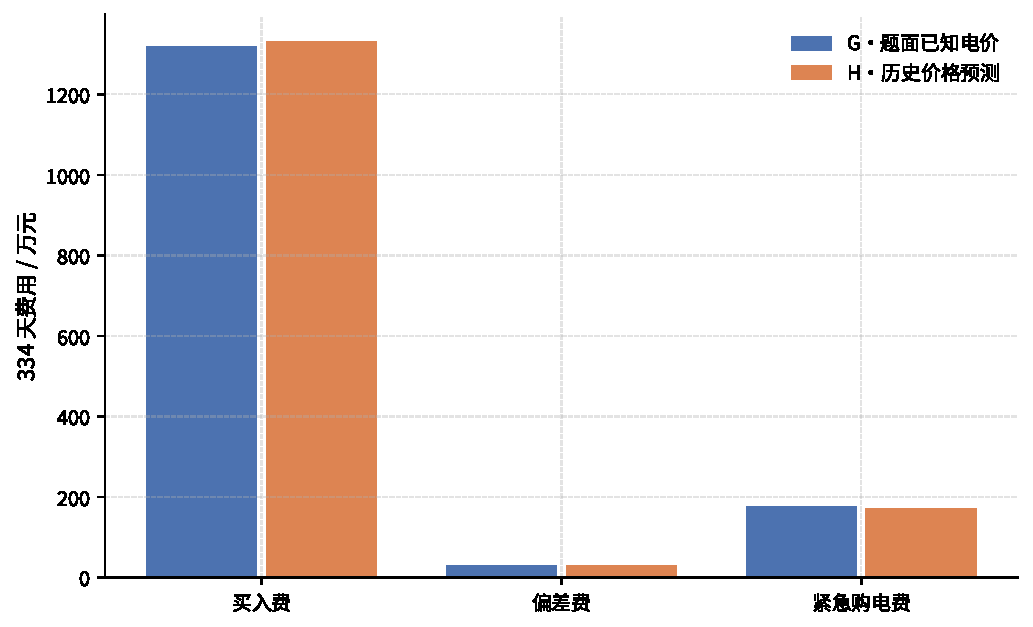
\includegraphics[width=.83\textwidth]{../../figures/Q4_调整层策略对比.pdf}
\caption{波动电价调整层在G、H两种信息条件下的费用分解}\label{fig:q4}
\end{figure}
以$I_p=(C_H-C_G)/C_G$度量条件电价信息价值，得到0.42\%和0.57\%。
该结果说明在这组数据及当前预测策略下，价格预测误差的额外成本较小；它不能推广为所有电价机制下的信息价值都很低。
G仍需面对未知的负荷与光伏，因此也不是所有不确定性消失后的理论最优下界。

\subsection{物理可行性与结果校验}
G无调整层和调整层的功率平衡最大残差分别为$4.547\times10^{-13}$与$3.411\times10^{-13}$ kWh，
SOC递推最大残差均为$1.137\times10^{-13}$ kWh；储电量落在1200至10800 kWh，同槽同时充放次数为0。
调整层正式方案不使用场景池。完整计划、最终调整、分段充放电与紧急购电事件分别写入题目指定的两份结果表。
\questionconclusion{波动价格条件下，无调整层费用1459.8万元，有调整层1410.3万元；历史电价预测扩展的额外费用分别为0.42\%与0.57\%。}

\section{灵敏度分析与一致性检验}
\subsection{已删除对冲扩展的稳定性}
为判断否定对冲是否只是某个随机种子的偶然结果，对已退出正式方案的候选扩展改变情景数、种子与历史池。
表\ref{tab:sens}取自独立灵敏度运行，参考配置为1349.3万元；本轮受控消融的对冲扩展为1349.2万元。
这一0.1万元差异不影响其均高于正式无对冲方案1347.1万元的判断；由于旧灵敏度缺少未舍入逐日记录，不擅自将差异归因为舍入。
\begin{table}[htbp]\centering
\caption{问题三灵敏度运行结果}\label{tab:sens}
\begin{tabular}{lrr}
\toprule
配置 & 费用/万元 & 相对灵敏度参考值\\\midrule
40情景，种子7（参考） & 1349.3 & 0\\
5情景，种子7 & 1350.4 & 0.08\%\\
10情景，种子7/17/27 & 1350.6/1350.4/1351.5 & 0.10/0.08/0.16\%\\
20情景，种子7/17/27 & 1349.2/1350.1/1349.3 & $-0.01$/0.06/0.00\%\\
40情景，种子17/27 & 1350.1/1349.0 & 0.06/$-0.02$\%\\
历史池回看30天 & 1351.3 & 0.15\%\\
历史池回看60天 & 1351.0 & 0.13\%\\
组合权重$\lambda=0.5$ & 1349.1 & $-0.01$\%\\
组合权重$\lambda=0.9$ & 1357.7 & 0.62\%\\
\bottomrule
\end{tabular}
\end{table}
40情景在不同种子下费用变化较小，但各变体并未给出稳定优于1347.1万元正式方案的证据。
短历史池略增费用，说明季节匹配与样本数量需平衡；该表只解释被删除扩展的行为，不再用于给正式策略选情景数。
$\lambda=0.9$明显较差，而0.5与0.7接近，支持保留历史预测成分。

\subsection{跨问题统一参数的代价}
既有问题三参数搜索是在对冲候选结构下完成，不能直接用于宣称无对冲正式方案的独立最优参数。
本轮保持$\lambda=0.7,\kappa=1.02,m=25$不变，只切换是否对冲，以保证消融可归因；其中$\kappa,m$仍沿用问题二开发期选定值，便于跨问比较。
冻结验证期仅用于判断对冲开关，没有反过来重选连续参数，从而避免重复利用验证集。
\subsection{信息与约束的分层检验}
实际执行按式\eqref{eq:discharge}--\eqref{eq:charge}由当前槽构成，结构上不读取未来实现值；残差池检查每个索引严格小于目标日；EWMA只吸收前一日及更早费用。
这些检查验证操作层面的因果性，但全局超参数使用2月至6月开发数据，开发期自身仍是拟合内评价。
另需区别场景LP的完整情景补救和在线因果控制，不能把情景目标值直接当作可实现结算值。

五份结果文件均通过工作表名、日期、行数、计划与紧急量汇总检查。
问题二和三的跨日SOC衔接最大误差为0，问题三计划费及计划量回读差为0；
紧急事件表因小数输出与相邻事件合并产生微小勾稽差，问题二约$2.300\times10^{-4}$ kWh，
问题三约$1.083\times10^{-3}$ kWh，远低于实际调度电量尺度。

\section{模型评价与推广}
\subsection{模型优点}
模型把购电结算、储能动态与信息发布时间统一起来。两日滚动使储能能够跨日转移，避免每晚回到固定电量所产生的人为限制；逐槽因果执行使每一步控制可由当时可得信息实现。
预测权重按历史费用更新，能响应非对称短缺惩罚；候选联合残差块保留负荷、光伏及日内相关结构，并经消融后未进入正式策略。
不同问题共用预测参数、评价区间和初值，有利于比较日内调整与电价信息的影响。

实证结果同时给出主方案、对照、消融与时间留出性能。无对冲更便宜、验证期最优不一定等于开发期最优等负结果被保留，使复杂模块的边际贡献可以检验。
\subsection{局限与改进方向}
首先，单年数据难以覆盖更广的气象与电价状态，100次重采样仅是条件压力评估。应增加独立年份或滚动多折验证，不能据本年度费用承诺未来节省。
其次，评价区间从2月开始，并以6000 kWh重新初始化。进一步研究应从题目给定的1月1日初值连续运行，再提取2月至12月结果，以排除初始化方式的影响。

第三，历史权重成本表仍以单日规划作代理；日内调整也只优化当日剩余时段，并使用零点规划产生的动态日末参考。
将权重标定和日内调整共同迁移到一致的多日滚动目标，可减少层间近似，但需要重新计算正式结果。
两日窗口的最远端尚无剩余电量价值函数，也可能出现窗口末端耗尽倾向；延长窗口或使用经验证的终端价值是值得比较的改进方案。

第四，实际执行器只针对当前缺口充放电，未显式考虑未来价格机会成本。
被删除的场景扩展采用整段情景补救，与在线执行存在信息差异；可进一步研究多阶段非预见性约束或价格感知的短窗实时控制。
最后，当前场景对冲没有表现出冻结验证期或全年降本优势，是否改善新增独立情景下的尾部风险仍需检验；储能衰减和购电容量上限也可在扩展模型中加入。
\subsection{结论}
典型日优化购电费为35126.95元，较无储能节省26.9\%。
在统一334天评价区间内，历史预测的两日滚动计划费用为1395.7万元；
加入组合预报与三点调整后，无对冲主方案为1347.1万元。
波动电价主口径下，两层费用分别为1459.8和1410.3万元。
这些结果支持跨日储能和日内更新的应用价值，同时说明评价复杂调度方法时，应将可执行性、实现费用、尾部风险和信息假设分别检验。

\begin{thebibliography}{99}
\bibitem{mayne2000}
Mayne D Q, Rawlings J B, Rao C V, Scokaert P O M.
Constrained model predictive control: Stability and optimality[J].
Automatica, 2000, 36(6): 789--814.
DOI: \href{https://doi.org/10.1016/S0005-1098(99)00214-9}{10.1016/S0005-1098(99)00214-9}.
\bibitem{huangfu2018}
Huangfu Q, Hall J A J. Parallelizing the dual revised simplex method[J].
Mathematical Programming Computation, 2018, 10(1): 119--142.
DOI: \href{https://doi.org/10.1007/s12532-017-0130-5}{10.1007/s12532-017-0130-5}.
\bibitem{rockafellar2000}
Rockafellar R T, Uryasev S. Optimization of conditional value-at-risk[J].
Journal of Risk, 2000, 2(3): 21--41.
DOI: \href{https://doi.org/10.21314/JOR.2000.038}{10.21314/JOR.2000.038}.
\end{thebibliography}

\begin{appendices}
\section{复现说明与关键执行步骤}
计算使用Python、NumPy、SciPy及HiGHS，结果表通过OpenPyXL回读。
运行环境提供 uv 与 requirements.txt 两种安装方式（详见支撑材料 README.txt）；正式Q3无场景随机性，对冲扩展种子为7、蒙特卡洛种子为42。复现时先进入随附Python工程目录。
命令及结果对应关系见表\ref{tab:repro}，求解中的微小正则项不计入正文购电费用。
\begin{table}[htbp]\centering
\caption{核心复现入口}\label{tab:repro}
\small
\begin{tabularx}{\textwidth}{p{.60\textwidth}X}
\toprule
命令 & 对应内容\\\midrule
\texttt{uv run python -m solve.q1} & 典型日调度\\
\texttt{uv run python -m solve.q2\_tune --result2} & 问题二正式结果\\
\texttt{uv run python -m solve.q3} & 问题三正式结果\\
\texttt{uv run python -m solve.q4\_price\_fit} & 历史电价成本标定\\
\texttt{uv run python -m solve.q4 --result4-2} & 波动价格无调整层\\
\texttt{uv run python -m solve.q4 --result4-3} & 波动价格调整层\\
\texttt{uv run python -m solve.q3\_ablation} & 正式方案与对冲扩展消融\\
\bottomrule
\end{tabularx}
\end{table}
复现顺序应先形成历史成本表与权重，再执行问题二和问题三，最后重算电价标定与问题四。
同一随机种子有助于比较方案，但线性规划的退化解、求解器版本和浮点阈值仍可能造成小规模数值差异。
\begin{lstlisting}[language=Python,basicstyle=\ttfamily\footnotesize,breaklines=true]
for day in evaluation_days:
    weights = update_from_past_costs(day)
    forecast = predict_two_days(day, weights)
    plan = optimize_horizon(forecast, actual_soc)
    for slot in current_day:
        if forecast_is_released(slot):
            commitment = adjust_remaining_plan(
                released_forecast, actual_soc, plan)
        load, pv = observe_current_slot(slot)
        charge, discharge, emergency, spill = execute(
            commitment[slot], load, pv, actual_soc)
        actual_soc += eta * charge - discharge / eta
    settle_day_and_export()
\end{lstlisting}
上述为算法逻辑说明，完整求解、时间映射和回读审计以随附源程序为准。
论文指定日期表直接取自正式Excel，计划量与调整量分别保留；紧急购电表列出全部对应事件，无事件日明确记为零。

\section{AI辅助说明}
本次论文整理使用AI编码助手辅助核对已有结果、组织公式和段落、生成表格与LaTeX排版。
数值依据为给定附件及随附求解程序输出，文献条目经公开来源核对。
此说明记录本次辅助范围，不替代参赛者对题意、模型与最终提交材料的审阅。

\end{appendices}
\end{document}
